\documentclass[12pt]{article}

\usepackage{url} % websites in bib
\usepackage{hyperref} 

\usepackage{graphicx} % images
\usepackage{subcaption}

\usepackage{amsmath} % formulas

\usepackage[]{algorithm2e} % pseudocode

\begin{document}
	\title{Skin detection in images using machine learning techniques for color and texture recognition}
	\author{Stefan Sebastian}
	\date{\today}
	\maketitle
	
	\begin{abstract}
		The interfaces between human and computer interaction have evolved from simple buttons to voice and video recognition. Skin detection is a useful preprocessing step for detecting people in images, which facilitates this communication. This article presents a method of detecting skin in images by combining several state of the art approaches in this domain. The model combines Skin Probability Maps for color analysis on images segmented with the Quick shift algorithm and texture detection using Haralick's features. The results, evaluated on the widely used Compaq dataset, are comparable to others found in literature: 80\% true positive rate and 20\% false positive rate.
	\end{abstract}
	
	\newpage
	\tableofcontents
	\newpage
	
	\section{Introduction}
	Skin detection means identifying pixels and regions in images which correspond to human skin. Starting from these regions we can build models that detect people or certain body parts.
	
	The purpose of this paper is to present the best models currently employed in skin detection and to propose a new model that combines some state of the art detectors. To the best of my knowledge no method that combines image segmentation, color and texture analysis has been published in this area of research.
	
	\section{Applications}
	One of the first applications in this field of study was scanning internet images in order to filter pornographic content \cite{finding_naked_people}. The model proposed in that paper scans the images for large areas of skin and then applies some geometrical analysis looking for elongated shapes.
	
	Another application was detecting anchorpersons in talk shows \cite{anchor_person_detection} for automatic annotation and storage. The data can be used for quickly finding videos containing specific persons or calculating how much time each anchorman was on stage.
	
	Skin detection is usually an intermediary step for detecting more concrete body parts, so I will also present some applications of those methods. Face and hands detection is used to facilitate human computer interaction. By scanning gestures and reactions a software system can respond in a more convenient way to the user. For example the Kinect camera, which connects to the Xbox console,
	allows the user to navigate menus using hand swipes \cite{kinect_control}. Face recognition, the next step after detection, is useful for automatic identification of people \cite{detecting_faces_a_survey} which has applications in security, such as unlocking your phone only when it scans your face, and monitoring certain areas, like the systems used by the Chinese government to fine jaywalkers caught on camera without human intervention \cite{jaywalkers_china}.
	
	\section{Related work}
	The subject of skin detection has been of interest for researchers due to its many applications. 
	
	\subsection{Skin Probability Maps}
	One of the most comprehensive experiments in skin detection was conducted by MJ Jones and JM Rehg \cite{compaq} who created the Compaq skin dataset, which became a standard for evaluating results of research in this domain.
	
	They used skin probability maps, which are histogram based models, meaning they set a number of bins for each color channel where they keep track of how many times each color pixel appears in the training set. Although \(256^3\) would be an obvious choice for the number of bins (one for each pixel) they determined that \(32^3\) is the optimum due to a large number of pixels not appearing in the training set. Each pixel is classified as being skin or non-skin using Bayes' theorem \(P(rgb|skin) >= \beta\), where $\beta$ is the threshold value. For this model they used a 6822 photo training set, where 4483 photos contained no skin and 2336 had portions of skin. The testing set had similar dimensions: 6818 total photos (4482 non-skin and 2336 skin). Using this method they obtained a 80\% true positive rate and 8.5\% false positive rate or, with a different threshold, a 90\% TP rate and 14.2\% FP rate.
	
	\subsection{Gaussian Models}
	Gaussian Models are probabilistic methods of representing skin distribution using Gaussian probability density functions. They rely on the assumption that skin pixels cluster in a small area of a color space \cite{survey_skin_color_modeling}.
	
	The previous paper \cite{compaq} also proposes a combination of two mixture models for skin and non-skin classes. Each model is composed of 16 gaussians and was trained on approximatively 74\% of the histogram data, because only that data was available at the time. The results were similar to those of the previous model: 80\%/9.5\% and 90\%/15.5\%.
	
	Lee and Yoo \cite{gaussian_applied} presented a Single Gaussian in CbCr space and a Gaussian Mixture in IQ space, both trained and tested on the Compaq dataset with the results of 90\%/33.3\% and 90\%/30\%, respectively.
	
	\subsection{Explicit thresholding}
	Thresholding is one of the fastest and simplest methods for skin detection. The basic idea is to define a set of rules and thresholds for the values of pixels in a given color space. This approach is best suited for real-time detection due to its speed. Some examples include \cite{rgb_threshold}, \cite{cr_cb_threshold}, \cite{yiq_threshold}, \cite{i_threshold} for face detection systems in different color spaces with varying results. 
	
	A set of thresholds for YCrCb space where proposed by Chai and Ngan\cite{cr_cb_threshold}. They set the ranges for Cb from 77 to 127 and for Cr from 133 to 173 and worked with the ECU database.
	
	Dai and Nakano\cite{yiq_threshold} created a model for YIQ, an orthogonal color space, which only used the I component (which stands for in-phase). The range they provided was [0, 50], however most of the images in their databases where of people with yellow skin.
	
	Brand and Mason \cite{i_threshold_applied} applied the technique from \cite{i_threshold}, which uses the YI'Q' space with the following threshold \(14 < I' < 40\), on the Compaq dataset and obtained 94.7\% TP rate and 30.2\% FP rate.
	
	An interesting approach, proposed by Gomez and Morales\cite{rca_threshold}, is having a learner find these rules automatically. They use RCA, a constructive induction algorithm, to build rules expressed with simple arithmetic operations in the rgb space. Their method achieves better results than the Bayesian SPM on their dataset, however it is computationally slower. The strategy implemented for RCA was finding attributes which cover either a large number of true positives or a few false positives. The starting attributes where r, g, b and the constant 1/3, which would generate new attributes using the operators : +, *, - and squaring. One of the best performing and simplest looking of the generated models looks like this:
	\begin{equation}
	\begin{split}
	\frac{r}{g} > 1.185 \quad \textrm{and}\\
	\frac{r * b}{(r + g + b)^2} > 0.107 \quad \textrm{and}\\
	\frac{r * g}{(r + g + b)^2} > 0.112
	\end{split}
	\end{equation}
	In comparison with the C4.5 decision tree algorithm, the RCA method obtained slightly worse results but with much simpler rules. They used a custom dataset containing images of more than 2000 people and obtained around 90\% both in precision and recall.
	
	\subsection{Models using segmentation}
	Frerk and Al-Hamadi\cite{superpixels_applied_1} proposed a method that applies image segmentation combined with a Bayesian SPM. The first step is calculating the probability for each pixel in an image and creating \(P_I\), the pixel probability image. \(P_I\) is used as input for a SLIC algorithm that calculates the superpixels. A probability is then computed for each superpixel and compared to a threshold.
	
	In \cite{superpixels_applied_2} a similar approach to \cite{superpixels_applied_1} is taken. Firstly, a segmentation is performed and superpixels are extracted. A probability is calculated for each superpixel as the average of its component pixels probabilities. Then, a CRF(Conditional Random Field) method is used in order to obtain smoother skin regions. This model was tested on the Compaq database and obtained a 91.17\% TP rate and 13.12\% FP rate.
	
	\subsection{Models using textural features}
	\cite{color_texture_ann} presents a model based on Artificial Neural Networks that analyzes both color and textural features. The color features used are the mean color, the standard deviation and the skewness. These are calculated for each channel (R, G, B). The inputs for the ANN also include the following textural information: Entropy, Energy, Contrast and Homogeneity, which are computed from the Gray-Level Co-Occurrence Matrix. The networks has three layers: an input layer, a hidden layer (with 50 neurons) and an output layer. The model was trained on 300 images (80x80 px) of skin and non-skin textures and tested on 100, obtaining a 96\% accuracy in classifying whether an image is a skin patch or not.
	
	Medjram et al.\cite{texture_svm} proposed another method that combines color and texture information. The first step is converting the initial image to the YCbCr color space. Skin regions are identified using thresholding like the following: \(77 <= Cb <= 127, 133 <= Cr <= 173\). Secondly, the image is sharpened in order to enhance its texture. The features considered from the GLCM are Contrast, Homogeneity and Energy, calculated over a 5x5 matrix. The last step is applying a Support Vector Machine classifier on the initial image to classify texture patches.
	
	In \cite{texture_gabor_wavelet} they use Gabor wavelet transforms to compute textural attributes. After identifying the initial skin regions a watershed segmentation algorithm is applied to increase true acceptance rate.
	
	\subsection{Hidden Markov Models}
	Sigal et al.\cite{hmm} implemented a method for real time skin detection in videos. Their model predicts the evolution of the skin color histogram using a second order Markov model, using an initial prediction from a Bayes classifier over the Compaq dataset. It uses the EM algorithm which consists of two steps: E(frame segmentation based on histogram) and M(histogram adaptation based on feedback from the current frame).
	
	\section{Proposed model}
	The model proposed by this paper is made up of three steps. The first step is image segmentation, which aims to divide the input image into several regions, called superpixels, based on color and shape. A Bayesian probability is then calculated for every pixel in the region and the average of these is compared to a threshold to determine if the superpixel's color is likely to be that of skin. Finally, a Support Vector Machine analyzes patches around each pixel and calculates Haralick features in order to classify the texture. The results from color and texture detection are then combined into the final result.
	
	\subsection{Datasets}
	For this experiment I have used two databases. First, the Compaq dataset \cite{compaq}, which is one of the most cited in literature, contains ~13.000 images out of which ~4700 contain skin and was used for the skin color model. The images were downloaded using a web crawler then divided into skin and non-skin images. For every skin image a black and white mask was created by hand to mark the regions of interest.
	
	The second dataset, SFA \cite{sfa}, was created as a combination of FERET(876 images) and AR(242 images)  datasets. It contains skin and non-skin patches of dimension from 1x1 to 35x35, which makes it ideal for the texture model. For each dimension, SFA has 3354 skin images and 5590 non-skin images.
	
	\subsection{Segmentation}
	Image segmentation has been applied to increase smoothness and eliminate holes in regions classified as skin. The algorithm chosen for image segmentation is Quick shift due to its simplicity, speed and its ability to form clusters without knowing their number beforehand.
	
	A suitable feature space for image segmentation is the combination of RGB components and pixel position, which can be scaled\cite{quickshift_gpu}. The algorithm starts by calculating a Parzen density value for each data point. Then it links each pixel to the nearest neighbor with a higher density. To obtain the regions we can limit our search during linking phase to a distance of \(\tau\). When calculating the density we can limit our search to a 3$\sigma$ window because the contributions for pixels further away should be small \cite{quickshift_gpu}.
	
	\begin{algorithm}
		\caption{The Quick shift segmentation algorithm from \cite{quickshift_gpu}}
		\label{alg:quick_shift}
		\# density computation\;
		\For{x in all pixels}{
			P[x] = 0\;
			\For{n in all pixels less than 3 * $\sigma$ away}{
				P[x] += exp(-(f[x] - f[n])\^{}2 / (2 * $\sigma$ * $\sigma$))	
			}
		}
		\# neighbor linking\;
		\For{x in all pixels}{
			\For{n in all pixels less than $\tau$ away}{
				\If{P[n] \(>\) P[x] and distance(x, n) is smaller than to previous parent}{
					d[x] = distance(x, n)\;
					parent[x] = n\;
				}
			}
		}
	\end{algorithm}

	\subsection{Color analysis}
	Each superpixel is evaluated with a color detection model. The chosen model is a Bayesian Skin Probability Map, due to its simplicity and speed. After scanning the input images we can calculate the following features: the number of skin pixels and non-skin pixels and the number of apparitions as skin and non-skin for each pixel. To determine whether a pixel can be classified as skin we can apply Bayes' Theorem as follows: \(p = P(X|S) * P(S) / P(X)\), where P(S), P(X) and P(X$\vert$S) represent the probabilities of finding a skin pixel, the selected pixel and the selected pixel given skin, respectively.
	
	The authors of the Compaq \cite{compaq} dataset made the observation that 77\% of the RGB space is empty and as a solution computed the probabilities on groups of pixels. The proposed model uses a similar method by taking the maximum probability in an area around the given pixel. This ensures that the considered pixel is always at the center of the group.
	
	\subsection{Texture analysis}
	Texture analysis is an independent step whose result is combined with that of the color detector's. Texture, while easily identifiable by a human observer, does not have precise definition. Consequently there are many choices for building a texture classification model depending on the author's interpretation.
	
	The chosen method for this model is the one proposed by Haralick \cite{haralick_features}. Features that describe texture are extracted from a matrix called the Gray Level Co-occurence Matrix, which represents how often combinations of pixel gray levels at different offsets appear in an image. A Support Vector Machine is trained on these features extracted from 5x5 patches. Each pixel is classified by building a window of the same size around it and giving that patch as input to the classifier.
	
	\subsection{Parameters}
	For image segmentation I tried to find values for the sigma and tau parameters that produce regions as large as possible without distorting the contours. I chose the (3, 5) pair, which can be seen in comparison with other pairs in figure \ref{fig:segmentation}.
	
	\begin{figure}[h!]
		\centering
		\begin{subfigure}[b]{0.3\linewidth}
			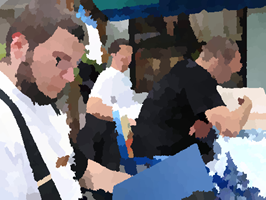
\includegraphics[width=\linewidth]{resources/segm_3_5.png}
			\caption{$\sigma = 3, \tau = 5$}
		\end{subfigure}
		\begin{subfigure}[b]{0.3\linewidth}
			
\includegraphics[width=\linewidth]{resources/segm_2_10.png}
			\caption{$\sigma = 2, \tau = 10$}
		\end{subfigure}
		\begin{subfigure}[b]{0.3\linewidth}
			
\includegraphics[width=\linewidth]{resources/segm_4_8.png}
			\caption{$\sigma = 4, \tau = 8$}
		\end{subfigure}
		\caption{Segmenting an image with different parameters}
		\label{fig:segmentation}
	\end{figure}

	The most suitable area for texture analysis was also determined experimentally. As can be observed in figure \ref{fig:texture} the 5x5 window offers a good detection of skin areas while the true positive rate goes down drastically for larger ones.
	
	\begin{figure}[h!]
		\centering
		\begin{subfigure}[b]{0.3\linewidth}
			
\includegraphics[width=\linewidth]{resources/texture_5_5.png}
			\caption{5x5}
		\end{subfigure}
		\begin{subfigure}[b]{0.3\linewidth}
			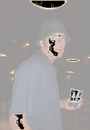
\includegraphics[width=\linewidth]{resources/texture_7_7.png}
			\caption{7x7}
		\end{subfigure}
		\begin{subfigure}[b]{0.3\linewidth}
			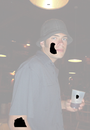
\includegraphics[width=\linewidth]{resources/texture_35_35.png}
			\caption{35x35}
		\end{subfigure}
		\caption{Texture detection with different windows}
		\label{fig:texture}
	\end{figure}
	
	I tried building color models in RGB, HSV and YCrCb and concluded that Bayesian color analysis obtains roughly the same results regardless of the color space chosen. For every pixel, I chose the maximum probability on a distance of 4 (similar to the bin size used in \cite{compaq}) on every feature. The threshold value can be used to control the TPR/FPR ratio.
	 
	\subsection{Evaluation}
	The model was evaluated on the Compaq skin database in order to compare it with other approaches from literature. There is a difference however, in the number of images chosen for evaluation. While most references use a ~6000 image set for testing I used only 50 images due to time constraints.
	
	For each image in the testing set I calculated the True Positive Rate and the False Positive Rate by comparing each pixel from my output to the given mask and then I averaged the results.
	\begin{equation}
	\label{metrics}
		TPR = \frac{TP}{TP + FN}, \,\,\, FPR = \frac{FP}{FP + TN}
	\end{equation}
	Equation \ref{metrics} shows how those metrics were calculated. TP, FP, TN and FN stand for the numbers of true positives, false positives, true negatives and false negatives, respectively.
	
	\begin{table}[h!]
		\begin{center}
			\caption{Evaluation of the proposed model on the Compaq dataset}
			\label{tab:results}
			\begin{tabular}{c|c|c}
				\textbf{TPR} & \textbf{FPR} & \textbf{Threshold}\\
				\hline
				86.57\% & 28.48\% & 0.1\\
				76.29\% & 15.54\% & 0.25\\
				81.59\% & 21.29\% & 0.167\\
			\end{tabular}
		\end{center}
	\end{table}
	
	\section{Conclusions}
	The model obtains results similar to the ones presented in literature however image segmentation and analyzing probabilities for every pixel's neighbors take a toll on computation speed. Due to time limitations, the evaluation was done on a small subset of the data. Consequently the model's performance might improve over a larger set of input data.
	
	\newpage
	\bibliography{references_articol}
	\bibliographystyle{ieeetr}
\end{document}